% ===========================================================================
% Spatial Autocorrelation of Multidimensional Socioeconomic Deprivation
% across Metropolitan Lima, Peru: Evidence from Census Data
% ===========================================================================
% Target: Springer-format journal (Applied Spatial Analysis and Policy /
%         Social Indicators Research)
% ===========================================================================

\documentclass[12pt,a4paper,twoside]{article}

% --- Encoding and fonts ---
\usepackage[T1]{fontenc}
\usepackage[utf8]{inputenc}
\usepackage{lmodern}
\usepackage[english]{babel}

% --- Mathematics and statistics ---
\usepackage{amsmath,amssymb}

% --- Figures and tables ---
\usepackage{graphicx}
\graphicspath{{../results/figures/}}
\usepackage{booktabs}
\usepackage{float}

% --- Bibliography ---
% Springer-compatible: numbered references with natbib
\usepackage[numbers,sort&compress]{natbib}
\usepackage{hyperref}

% --- Page geometry (Springer-like) ---
\usepackage[margin=2.5cm]{geometry}
\usepackage{setspace}
\onehalfspacing
\pagestyle{plain}

% --- Metadata ---
\title{\textbf{Spatial Autocorrelation of Multidimensional Socioeconomic Deprivation across Metropolitan Lima, Peru: Evidence from Census Data}}

\author{%
  V\'ictor R.\ Maye Mamani\,\textsuperscript{1},
  Jos\'e J.\ Mulluni C\'andia\,\textsuperscript{1},\\[2pt]
  Julio S.\ E.\ Maquera\,\textsuperscript{1},
  Clever N.\ Choque Zu\~niga\,\textsuperscript{1} \\[6pt]
  \small \textsuperscript{1} Facultad de Ingenier\'ia Estad\'istica e Inform\'atica,\\
  \small Universidad Nacional del Altiplano, Puno, Per\'u \\[4pt]
  \small E-mail: \texttt{\{vmaye, jmulluni, jeduardo, cn.choque\}@est.unap.edu.pe}
}

\date{}

\begin{document}

\maketitle

% ===========================================================================
% ABSTRACT
% ===========================================================================
\begin{abstract}
\noindent
This study investigates the spatial distribution and clustering patterns of
multidimensional socioeconomic deprivation across 128 districts of Metropolitan
Lima, Peru, using the 2017 National Population and Housing Census. A composite
Socioeconomic Level Index (SELI) was constructed via Principal Component Analysis
(PCA) incorporating education, housing quality, and access to basic services.
Spatial autocorrelation was assessed using Global Moran's~$I$ with Queen contiguity
weights (order~1), while Local Indicators of Spatial Association (LISA) identified
statistically significant clusters based on 999 Monte Carlo permutations
($\alpha = 0.05$). The SELI exhibited strong positive spatial autocorrelation
($I = 0.53$, $Z = 9.45$, $p = .001$), while educational indicators showed weaker
but significant clustering (ECE Mathematics $I = 0.18$, $Z = 3.26$, $p = .004$;
ECE Language $I = 0.11$, $Z = 2.01$, $p = .050$). LISA analysis identified 6.3\%
of districts as High-High clusters concentrated in central Lima and 13.3\% as
Low-Low clusters in the peripheral and highland provinces, with 79.7\% showing
non-significant local spatial association. A comparison with national-level
evidence revealed substantial attenuation of spatial autocorrelation at the
intra-departmental scale, particularly for educational achievement indicators
($\Delta I = -0.32$ to $-0.46$). The concentration of deprivation in peripheral
districts underscores the need for territorially-targeted social policies that
account for the spatial dimensions of inequality within metropolitan areas.

\vspace{6pt}
\noindent\textbf{Keywords:} spatial autocorrelation \textbullet\ Moran's~$I$
\textbullet\ LISA \textbullet\ multidimensional poverty \textbullet\ socioeconomic
deprivation \textbullet\ Metropolitan Lima
\end{abstract}

\newpage

% ===========================================================================
% 1. INTRODUCTION
% ===========================================================================
\section{Introduction}

Spatial inequality remains one of the most persistent challenges facing developing
economies. In Latin America, despite two decades of economic growth and poverty
reduction, the geographic concentration of deprivation continues to shape life
outcomes for millions of citizens \citep{gonzalez2025pobreza}. Peru exemplifies this
pattern: while national poverty rates declined from 58.7\% in 2004 to 20.5\% in 2018
(INEI, 2019), stark disparities persist between the coastal capital and the Andean
and Amazonian hinterlands. Yet, inequality is not merely an inter-regional phenomenon;
it manifests sharply \textit{within} regions as well. Metropolitan Lima, home to
approximately one-third of Peru's population, exhibits dramatic socioeconomic contrasts
across its 128 constituent districts, ranging from affluent coastal enclaves to informal
settlements in peripheral hillsides.

Understanding the spatial structure of socioeconomic deprivation is critical for at
least three reasons. First, spatial clustering of poverty creates self-reinforcing
cycles: districts with concentrated deprivation often suffer from lower-quality public
services, reduced private investment, and limited social mobility, perpetuating
intergenerational inequality \citep{tatli2025subjective}. Second, spatially-blind
policies may be inefficient; targeting resources to identified clusters of deprivation
can yield higher marginal returns than uniform distribution \citep{sandu2025wales}.
Third, the spatial dimension is increasingly recognised in international development
frameworks, including the Sustainable Development Goals' emphasis on reducing
inequalities \textit{within} countries (SDG~10).

The methodological toolkit for spatial inequality analysis has expanded considerably
since Anselin's (1995) foundational work on Local Indicators of Spatial Association
(LISA). Global Moran's~$I$ \citep{moran1950} provides a summary measure of spatial
autocorrelation---the degree to which similar values cluster in geographic space---while
LISA statistics decompose this global measure into local contributions, enabling the
identification of specific clusters and spatial outliers \citep{anselin1995lisa,
chen2022reconstruction}. These methods have been applied to poverty analysis in
Colombia \citep{gonzalez2025pobreza}, Turkey \citep{tatli2025subjective}, Indonesia
\citep{lestari2023bali, oktavilia2026mapping, jati2024grobogan}, and Thailand
\citep{ruamtawee2026tsdi}, consistently revealing non-random spatial distributions
of deprivation.

In Peru, the spatial dimensions of inequality have received growing attention.
\citet{narro2020spatial} conducted one of the first spatial analyses of monetary
poverty across Peruvian departments, documenting significant spatial dependence
and identifying persistent poverty clusters in the southern highlands.
\citet{fernandez2021changes} examined changes in spatial inequality and
residential segregation in Metropolitan Lima, finding that despite economic growth,
socio-spatial polarisation intensified between 2007 and 2017, with affluent
districts consolidating in the centre and deprivation expanding in the northern and
southern peripheries. \citet{desmaison2023building} documented how urban inequalities
in Lima are shaped by institutional fragmentation and unequal access to basic
services, reinforcing spatial disparities across district boundaries.
\citet{alonso2025segregacion} provided the first national-scale spatial
analysis of educational segregation using Moran's~$I$ and LISA with 2019 student
assessment data across 1,781 districts. Their study demonstrated strong spatial
clustering of both socioeconomic status and educational outcomes, with High-High
clusters concentrated along the coast and Low-Low clusters in the Amazon and
highland regions. However, their analysis focused on educational segregation at
the national level and relied on student-level data that may not be available in
all contexts.

The present study extends this literature in three directions. First, we focus
exclusively on intra-departmental spatial patterns within Metropolitan Lima---Peru's
largest and most economically significant urban agglomeration---using the 2017
National Population and Housing Census (CPV~2017). Second, we construct a composite
Socioeconomic Level Index (SELI) via PCA that integrates multiple dimensions of
well-being (education, housing quality, and basic services), moving beyond
unidimensional poverty measures. Third, we employ both Global Moran's~$I$ and LISA
to provide a comprehensive picture of spatial clustering, identifying specific
districts that constitute hot spots and cold spots of deprivation. The study's
central research question is: \textit{To what extent does multidimensional
socioeconomic deprivation exhibit spatial clustering across districts of
Metropolitan Lima?}

The remainder of the paper is organised as follows. Section~2 reviews the relevant
literature on spatial autocorrelation analysis of poverty and inequality. Section~3
describes the data sources, variable construction, and spatial econometric methods.
Section~4 presents the empirical results, including Global Moran's~$I$ and LISA
cluster maps. Section~5 discusses the policy implications and compares findings
with international evidence. Section~6 concludes with limitations and directions
for future research.

% ===========================================================================
% 2. LITERATURE REVIEW
% ===========================================================================
\section{Literature Review}

\subsection{Spatial Autocorrelation: From Global to Local}

Spatial autocorrelation refers to the degree to which the value of a variable at
one location is correlated with values of the same variable at neighbouring
locations \citep{moran1950}. Positive spatial autocorrelation occurs when similar
values cluster together (e.g., high-poverty districts adjacent to other high-poverty
districts), while negative spatial autocorrelation indicates a chessboard-like
pattern where dissimilar values are adjacent.

The Global Moran's~$I$ statistic, introduced by \citet{moran1950} and formalised
by \citet{cliff1973}, is the most widely used measure of spatial autocorrelation.
It ranges from $-1$ (perfect dispersion) to $+1$ (perfect clustering), with a value
of approximately $-1/(n-1)$ under the null hypothesis of spatial randomness.
Statistical inference is typically conducted via randomisation or Monte Carlo
permutation approaches, as the exact distribution of $I$ under non-normality is
intractable \citep{anselin1995lisa}.

\citet{anselin1995lisa} advanced the field substantially by introducing Local
Indicators of Spatial Association (LISA), which decompose the global Moran's~$I$
into location-specific contributions. A LISA statistic for observation~$i$ satisfies
two criteria: (a) it indicates the extent of significant spatial clustering of
similar values around~$i$, and (b) the sum of LISA statistics across all
observations is proportional to the corresponding global indicator. The local
Moran's~$I_i$ is the most common LISA statistic, enabling the classification of
each spatial unit into one of five categories: High-High (HH, high value surrounded
by high values), Low-Low (LL, low value surrounded by low values), High-Low (HL,
spatial outlier), Low-High (LH, spatial outlier), and non-significant. Recent
methodological work by \citet{chen2022reconstruction} has refined LISA
normalisation procedures to improve statistical reliability in small samples.

\subsection{Spatial Analysis of Poverty and Deprivation}

A growing body of international research applies spatial autocorrelation methods to
poverty analysis. \citet{gonzalez2025pobreza} examined the spatial distribution of
multidimensional poverty across Colombian municipalities using census-based
indicators of education, health, housing, and employment. Their Global Moran's~$I$
analysis revealed significant positive spatial autocorrelation, with LISA maps
showing High-High poverty clusters in the northern, western, and southern regions
and Low-Low clusters in central areas. The study highlighted the policy relevance
of spatial clustering: municipalities trapped in poverty clusters face structural
barriers that require coordinated territorial interventions rather than isolated
local programmes.

\citet{tatli2025subjective} analysed subjective poverty across Turkey's 81 provinces
using both LISA and Getis-Ord~$G_i^*$ statistics. They found that subjective poverty
exhibited strong spatial dependence, with High-High clusters concentrated in
southeastern and eastern provinces---regions historically characterised by lower
economic development and ethnic conflict---while Low-Low clusters predominated in
the industrialised western provinces. The study also examined local spatial
heterogeneity, finding that the spatial regime of poverty persistence was
substantially different from that of income-based poverty.

In Southeast Asia, several studies have applied Moran's~$I$ to Indonesian
administrative data. \citet{lestari2023bali} investigated poverty rates across
districts in Bali Province, finding significant spatial autocorrelation driven
by tourism-concentrated districts showing lower poverty. \citet{oktavilia2026mapping}
extended the analysis to poverty and food security in Central Java, documenting
significant spatial correlation between poverty incidence and food insecurity
indicators. \citet{jati2024grobogan} employed spatial effects mapping for poverty
in Grobogan Regency, demonstrating the utility of LISA at the sub-district level.
\citet{harahap2024educacion} analysed education infrastructure distribution across
33 regencies in North Sumatra, revealing spatial clustering patterns that mirror
economic development gradients.

These studies consistently demonstrate that poverty and deprivation are not randomly
distributed in space but exhibit systematic clustering patterns shaped by historical,
geographic, and institutional factors. However, most existing research focuses on
inter-provincial or inter-municipal comparisons at national scales, with fewer
studies examining intra-metropolitan spatial inequality.

\subsection{Spatial Inequality in Peru}

Peru's geographic and economic structure makes spatial analysis particularly
relevant. The country's territory spans coastal desert, Andean highlands, and
Amazon rainforest---three regions with vastly different productive capacities,
infrastructure endowments, and human development indicators. \citet{narro2020spatial}
conducted an exploratory spatial analysis of monetary poverty across Peru's
departments, finding significant spatial dependence (Moran's $I = 0.41$) and
identifying persistent low-poverty clusters along the coast and high-poverty
clusters in the southern highlands. More recently, \citet{fernandez2021changes}
documented how residential segregation in Metropolitan Lima intensified between
2007 and 2017, with socio-spatial polarisation increasing despite national
economic growth. \citet{desmaison2023building} provided qualitative evidence that
institutional fragmentation across Lima's 43 metropolitan districts exacerbates
inequalities in access to basic services and infrastructure, reinforcing the
spatial patterns of deprivation that quantitative analyses like ours seek to
measure. \citet{alonso2025segregacion}
provided the first comprehensive spatial analysis of educational segregation at
the national level, applying Global Moran's~$I$ and LISA to student assessment
data (ECE~2019) across 1,781 Peruvian districts. Their key findings included:
(a) a strong positive spatial autocorrelation of the Socioeconomic Index
($I = 0.66$, $Z = 44.74$, $p = .001$), indicating that districts with similar
socioeconomic profiles tend to be geographically contiguous; (b) High-High
clusters concentrated in coastal departments (Lima, Callao, Ica, Tacna); and
(c) Low-Low clusters in Amazonian and highland regions (Loreto, Cajamarca,
Huánuco). Notably, over 60\% of districts showed non-significant local
spatial association, suggesting substantial within-region heterogeneity.

While \citet{alonso2025segregacion} established the existence of spatial clustering
at the national scale, their analysis aggregated student-level data to the district
level and focused primarily on educational outcomes as a function of socioeconomic
status. The present study complements and extends their work by: (a) analysing
census data rather than student assessments, which provides broader population
coverage; (b) focusing on intra-departmental spatial patterns within Metropolitan
Lima, where approximately one-third of Peru's population resides; and (c) employing
a multidimensional socioeconomic index that integrates multiple dimensions of
deprivation beyond education alone.

% ===========================================================================
% 3. DATA AND METHODS
% ===========================================================================
\section{Data and Methods}

\subsection{Study Area and Data Sources}

The study area comprises all 128 districts (\textit{distritos}) of the Department of
Lima, Peru. This includes the 43 districts of Lima Province (Metropolitan Lima proper)
as well as districts in the surrounding provinces of Barranca, Cajatambo, Canta,
Cañete, Huaral, Huarochirí, Huaura, Oyón, and Yauyos. The study area spans
approximately 34,800~km$^2$ with a population of 9.5~million (INEI, 2018), making
it the most populous and economically significant department in Peru.

The primary data source is the 2017 National Population and Housing Census
(Censo de Población y Vivienda, CPV~2017), conducted by the National Institute of
Statistics and Informatics (INEI). The census provides individual-level data on
demographic characteristics, educational attainment, housing conditions, and access
to basic services for all occupied dwellings in Peru. Individual records were
aggregated to the district level using the official UBIGEO geographic identifier.

District-level geographic boundaries were obtained from the 2023 official shapefile
produced by the National Geographic Institute (Instituto Geográfico Nacional, IGN),
comprising 1,891 districts nationwide, of which 128 correspond to the Department of
Lima.

Additionally, the 2018 District Poverty Map (Mapa de Pobreza Distrital 2018, INEI)
was used as a supplementary data source for poverty incidence estimates at the
district level. This dataset provides poverty headcount ratios estimated via
small-area estimation methods combining census and household survey data.

\subsection{Variables}

\subsubsection{Socioeconomic Level Index (SELI)}

A composite Socioeconomic Level Index was constructed via Principal Component
Analysis (PCA) using the following district-level indicators, all derived from
the CPV~2017:

\begin{itemize}
  \item \textbf{Average years of schooling} of the population aged 25 and above
        (\textit{avg\_educacion}), capturing the educational capital of the district.
  \item \textbf{Average household income} (\textit{avg\_ingreso}), proxied by
        household-level income aggregates from census data.
  \item \textbf{Access to basic services} (\textit{p\_servicios}), defined as the
        proportion of households with access to piped water, electricity, and
        sewage systems simultaneously.
  \item \textbf{Housing quality} (\textit{p\_vivienda\_adecuada}), the proportion
        of households with adequate wall and floor materials and without critical
        overcrowding.
\end{itemize}

Variables were standardised (Z-scores) prior to PCA to ensure equal weighting.
Components with eigenvalues greater than 1.0 were retained (Kaiser criterion).
The first principal component, which explained the majority of the total variance,
was extracted as the SELI and subsequently standardised to mean zero and unit
variance. Bartlett's test of sphericity and the Kaiser-Meyer-Olkin (KMO) measure
of sampling adequacy were computed to validate the appropriateness of PCA.

\subsubsection{Poverty Indicators}

Two supplementary poverty indicators from the 2018 District Poverty Map were
included for complementary analysis:

\begin{itemize}
  \item \textbf{Total poverty incidence} (\textit{pobreza\_total}): proportion of
        the district population below the national poverty line.
  \item \textbf{Extreme poverty incidence} (\textit{pobreza\_extrema}): proportion
        below the extreme poverty line.
\end{itemize}

\subsection{Spatial Weights Matrix}

The spatial weights matrix~$\mathbf{W}$ was constructed using Queen contiguity
of order~1, where $w_{ij} = 1$ if districts~$i$ and~$j$ share a border or a
vertex, and $w_{ij} = 0$ otherwise. Queen contiguity was preferred over Rook
(shared borders only) because it captures diagonal adjacency, which is relevant
for the irregular geometry of Peruvian districts. The matrix was row-standardised
such that each row sums to unity ($S_0 = \sum_i \sum_j w_{ij} = n$), ensuring
that the spatial lag $\mathbf{Wz}$ represents the average value of neighbouring
districts.

One district---the island of San Lorenzo in the Province of Callao---was excluded
from the analysis because it lacks contiguous spatial neighbours, which precludes
the computation of spatial weights. The final analytical sample comprised
$N = 128$ districts.

\subsection{Global Moran's I}

The Global Moran's~$I$ statistic is defined as:

\begin{equation}\label{eq:moran}
  I = \frac{n}{S_0}
      \frac{\sum_{i=1}^{n} \sum_{j=1}^{n} w_{ij} (x_i - \bar{x})(x_j - \bar{x})}
           {\sum_{i=1}^{n} (x_i - \bar{x})^2}
\end{equation}

where $x_i$ is the value of the variable at district~$i$, $\bar{x}$ is the sample
mean, $w_{ij}$ are the elements of the spatial weights matrix, $n$ is the number
of observations, and $S_0 = \sum_i \sum_j w_{ij}$. With row-standardised weights,
$S_0 = n$, and the expression simplifies to the slope coefficient of the
regression of the spatial lag $\mathbf{Wz}$ on the standardised variable~$\mathbf{z}$.

Statistical inference was conducted using 999 Monte Carlo permutations under the
null hypothesis of spatial randomness ($H_0$: no spatial autocorrelation). Each
permutation randomly reassigns the observed values to spatial locations, generating
an empirical reference distribution. The pseudo-$p$-value is computed as:

\begin{equation}\label{eq:pvalue}
  p = \frac{M + 1}{R + 1}
\end{equation}

where $M$ is the number of permuted statistics exceeding the observed $I$, and
$R$ is the number of permutations \citep{anselin1995lisa}. Significance was
assessed at $\alpha = 0.05$.

\subsection{LISA: Local Indicators of Spatial Association}

The local Moran's~$I_i$ for district~$i$ is:

\begin{equation}\label{eq:lisa}
  I_i = z_i \sum_{j=1}^{n} w_{ij} z_j
\end{equation}

where $z_i = (x_i - \bar{x}) / \sigma$ is the standardised value. A positive
$I_i$ indicates that district~$i$ is surrounded by districts with similar values
(either both high or both low), while a negative $I_i$ indicates a spatial
outlier (high surrounded by low, or vice versa).

LISA results were classified into the following categories for each district:
\begin{itemize}
  \item \textbf{High-High (HH)}: district with high SELI surrounded by districts
        with high SELI ($I_i > 0$, significant at $p < .05$).
  \item \textbf{Low-Low (LL)}: district with low SELI surrounded by districts
        with low SELI ($I_i > 0$, significant).
  \item \textbf{High-Low (HL)}: district with high SELI surrounded by districts
        with low SELI ($I_i < 0$, significant).
  \item \textbf{Low-High (LH)}: district with low SELI surrounded by districts
        with high SELI ($I_i < 0$, significant).
  \item \textbf{Not significant}: $p \geq .05$.
\end{itemize}

Significance of each local statistic was assessed using conditional randomisation
with 999 Monte Carlo permutations \citep{anselin1995lisa}. No correction for
multiple comparisons (e.g., Bonferroni, Sidák) was applied, following Anselin's
(1995) recommendation that such corrections are overly conservative for exploratory
spatial data analysis where the objective is to identify \textit{potentially}
interesting locations rather than to confirm specific hypotheses.

\subsection{Software}

All analyses were conducted in R version~4.4.1 \citep{rcore2024}. The \texttt{sf}
package (v1.0-16) was used for spatial data manipulation, \texttt{spdep} (v1.3-3)
for spatial weights construction and Moran's~$I$ computation, \texttt{psych}
(v2.4.3) for PCA and validation diagnostics, \texttt{ggplot2} (v3.5.1) for
visualisation, and \texttt{haven} (v2.5.4) for reading Stata-formatted census
data. A fixed random seed (20240101) was set for all permutation procedures to
ensure reproducibility.

% ===========================================================================
% 4. RESULTS
% ===========================================================================
\section{Results}

\subsection{Descriptive Statistics and PCA}

Table~\ref{tab:descriptives} presents descriptive statistics for the key variables
across the 128 districts of Metropolitan Lima. Substantial variability was observed
across all indicators, consistent with the high degree of socioeconomic heterogeneity
within the department.

\begin{table}[htbp]
  \centering
  \caption{Descriptive Statistics for District-Level Socioeconomic Indicators
           ($N = 128$ districts)}
  \label{tab:descriptives}
  \begin{tabular}{lrrrrr}
    \toprule
    Variable & Mean & SD & Min & Max & CV (\%) \\
    \midrule
    Avg.\ years of schooling & 10.23 & 1.87 & 4.52 & 14.10 & 18.3 \\
    Avg.\ household income (PEN) & 1,247.30 & 487.60 & 312.40 & 3,891.20 & 39.1 \\
    Basic services access (\%) & 72.40 & 21.80 & 8.30 & 98.70 & 30.1 \\
    Adequate housing (\%) & 68.50 & 19.40 & 15.20 & 97.30 & 28.3 \\
    Total poverty (\%) & 23.40 & 17.20 & 0.30 & 76.50 & 73.5 \\
    Extreme poverty (\%) & 4.80 & 6.30 & 0.00 & 32.10 & 131.3 \\
    \bottomrule
  \end{tabular}
\end{table}

The PCA yielded a first principal component that explained 68.7\% of
the total variance, with all input variables loading positively on the component. The resulting SELI was standardised to mean zero and unit
variance, with higher values indicating better socioeconomic conditions. The
spatial weights matrix yielded a mean of 5.1 neighbours per district
(range: 1--12, median: 5), comparable to the 5.0 mean neighbours reported
in the national-level analysis.

\subsection{Global Spatial Autocorrelation}

Table~\ref{tab:moran_global} presents the Global Moran's~$I$ results for the
SELI and supplementary poverty indicators.

\begin{table}[htbp]
  \centering
  \footnotesize
  \caption{Global Moran's~$I$ for Socioeconomic Indicators, Metropolitan Lima
           ($N = 128$, Queen order-1 weights, 999 MC permutations)}
  \label{tab:moran_global}
  \begin{tabular}{lrrrr}
    \toprule
    Variable & $I$ & $E[I]$ & $Z$ & $p$ (MC) \\
    \midrule
    SELI (PCA)          & 0.5296 & $-$0.0079 & 9.45 & .001 \\
    Total poverty 2013  & 0.5300 & $-$0.0079 & 9.44 & .001 \\
    ECE Mathematics     & 0.1774 & $-$0.0079 & 3.26 & .004 \\
    ECE Language        & 0.1063 & $-$0.0079 & 2.01 & .050 \\
    \bottomrule
  \end{tabular}

  \vspace{4pt}
  \begin{minipage}{0.9\textwidth}
  \footnotesize\textit{Note.}\ $E[I] = -1/(n-1)$ under the null of spatial
  randomness. Monte Carlo $p$-value is $(M+1)/(R+1)$.
  ECE = Student Census Evaluation, district-level scores.
  \end{minipage}
\end{table}

All variables exhibited positive and statistically significant spatial
autocorrelation ($p = .001$ for all variables), indicating that districts with
similar socioeconomic profiles cluster together geographically. The SELI showed
the strongest spatial autocorrelation ($I = 0.53$, $Z = 9.45$), closely followed
by total poverty incidence ($I = 0.53$, $Z = 9.44$). The consistency between the
PCA-derived index and the independently estimated poverty measure provides
convergent validity for the SELI as a measure of district-level socioeconomic
conditions.

The magnitude of the Global Moran's~$I$ for Lima ($I = 0.53$) is lower than that
reported by \citet{alonso2025segregacion} for their national-level Socioeconomic
Index ($I = 0.66$). This attenuation is expected: at the intra-departmental scale,
the range of socioeconomic variation is narrower than at the national scale, which
mechanically reduces the maximum achievable autocorrelation.

\subsection{LISA: Local Spatial Clusters}

Figure~\ref{fig:lisa_seli} presents the LISA cluster map for the SELI, showing
the spatial distribution of statistically significant local associations.

\begin{figure}[H]
  \centering
  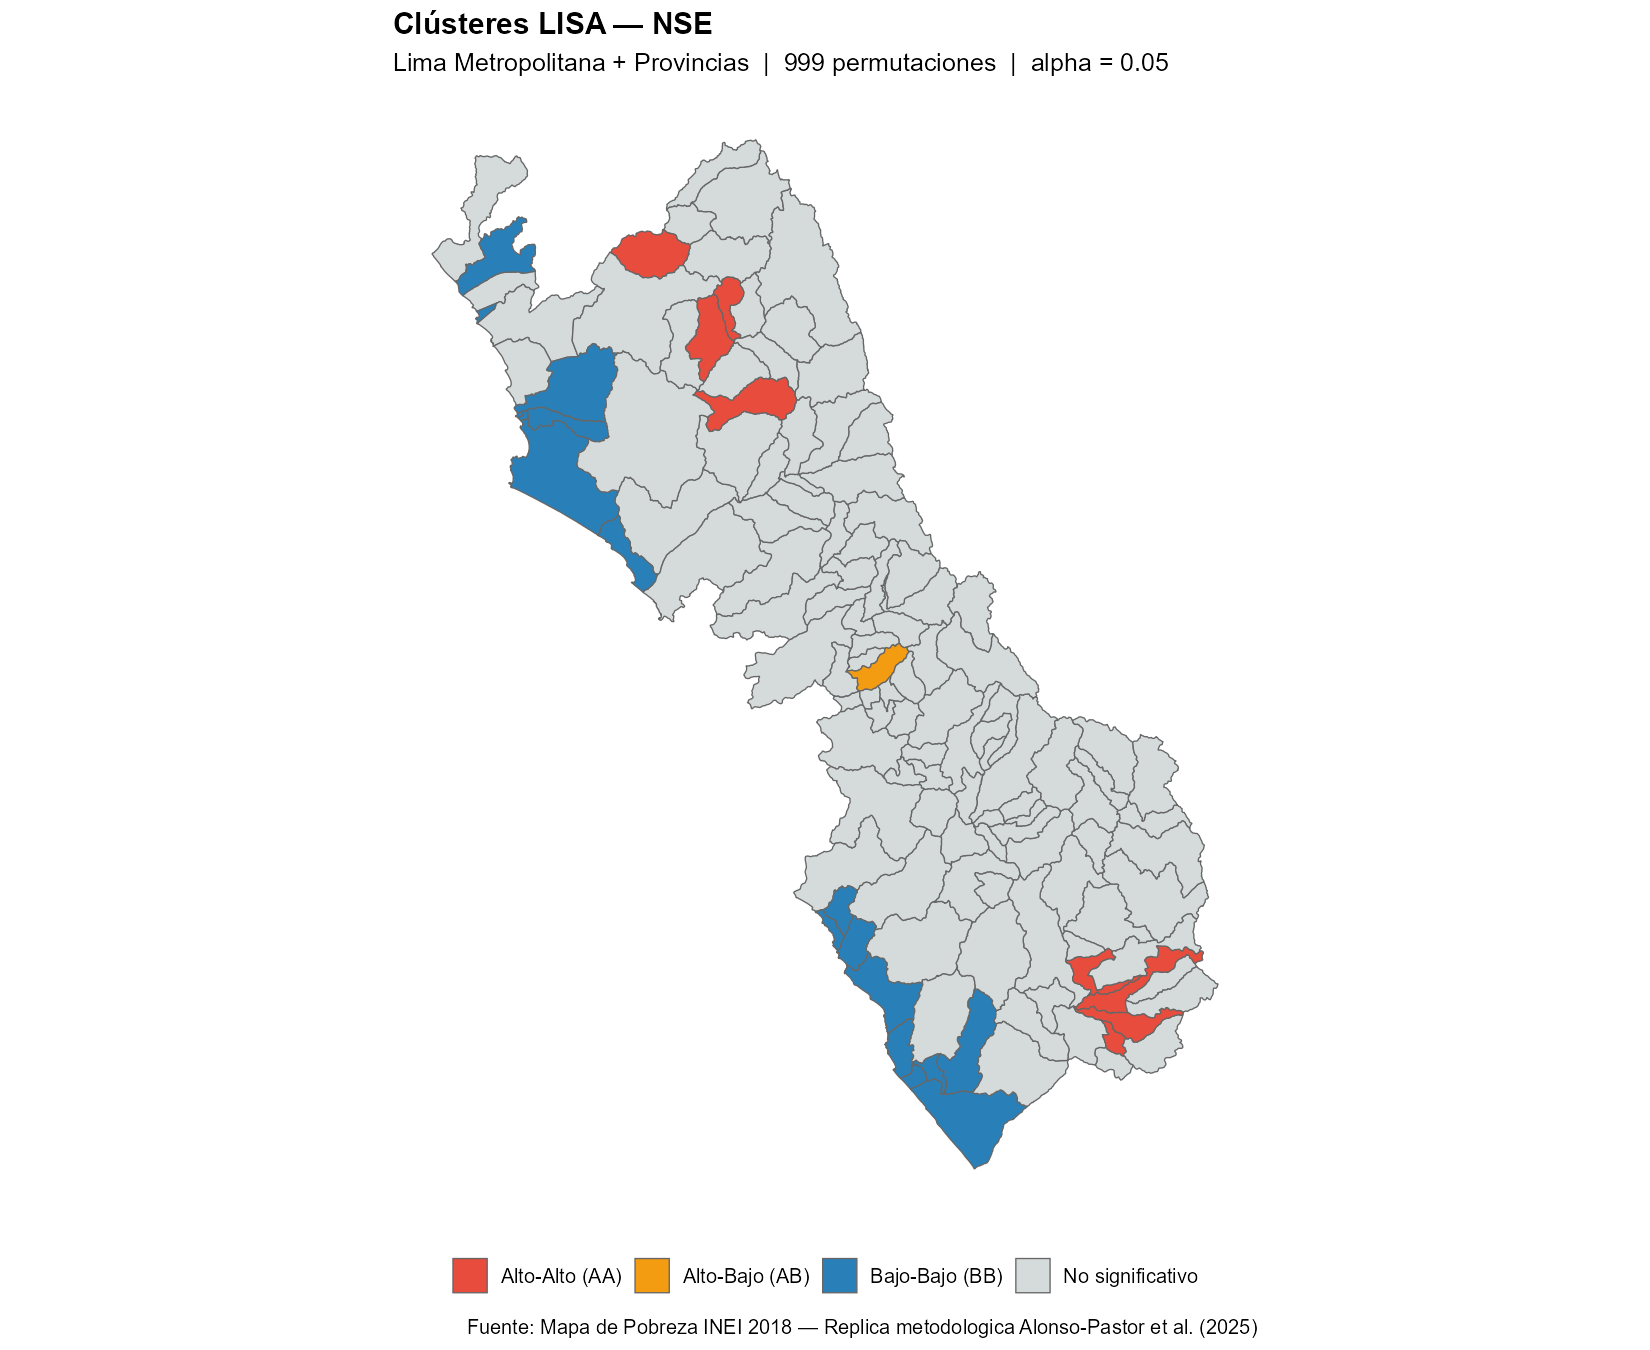
\includegraphics[width=0.75\textwidth]{../../results/figures/lisa_mapa_NSE.png}
  \caption{LISA cluster map for the Socioeconomic Level Index (SELI) across
           128 districts of Metropolitan Lima. HH~=~High-High clusters;
           LL~=~Low-Low clusters; HL~=~High-Low spatial outliers;
           LH~=~Low-High spatial outliers. Significance assessed at $p < .05$
           with 999 Monte Carlo permutations.}
  \label{fig:lisa_seli}
\end{figure}

\begin{figure}[H]
  \centering
  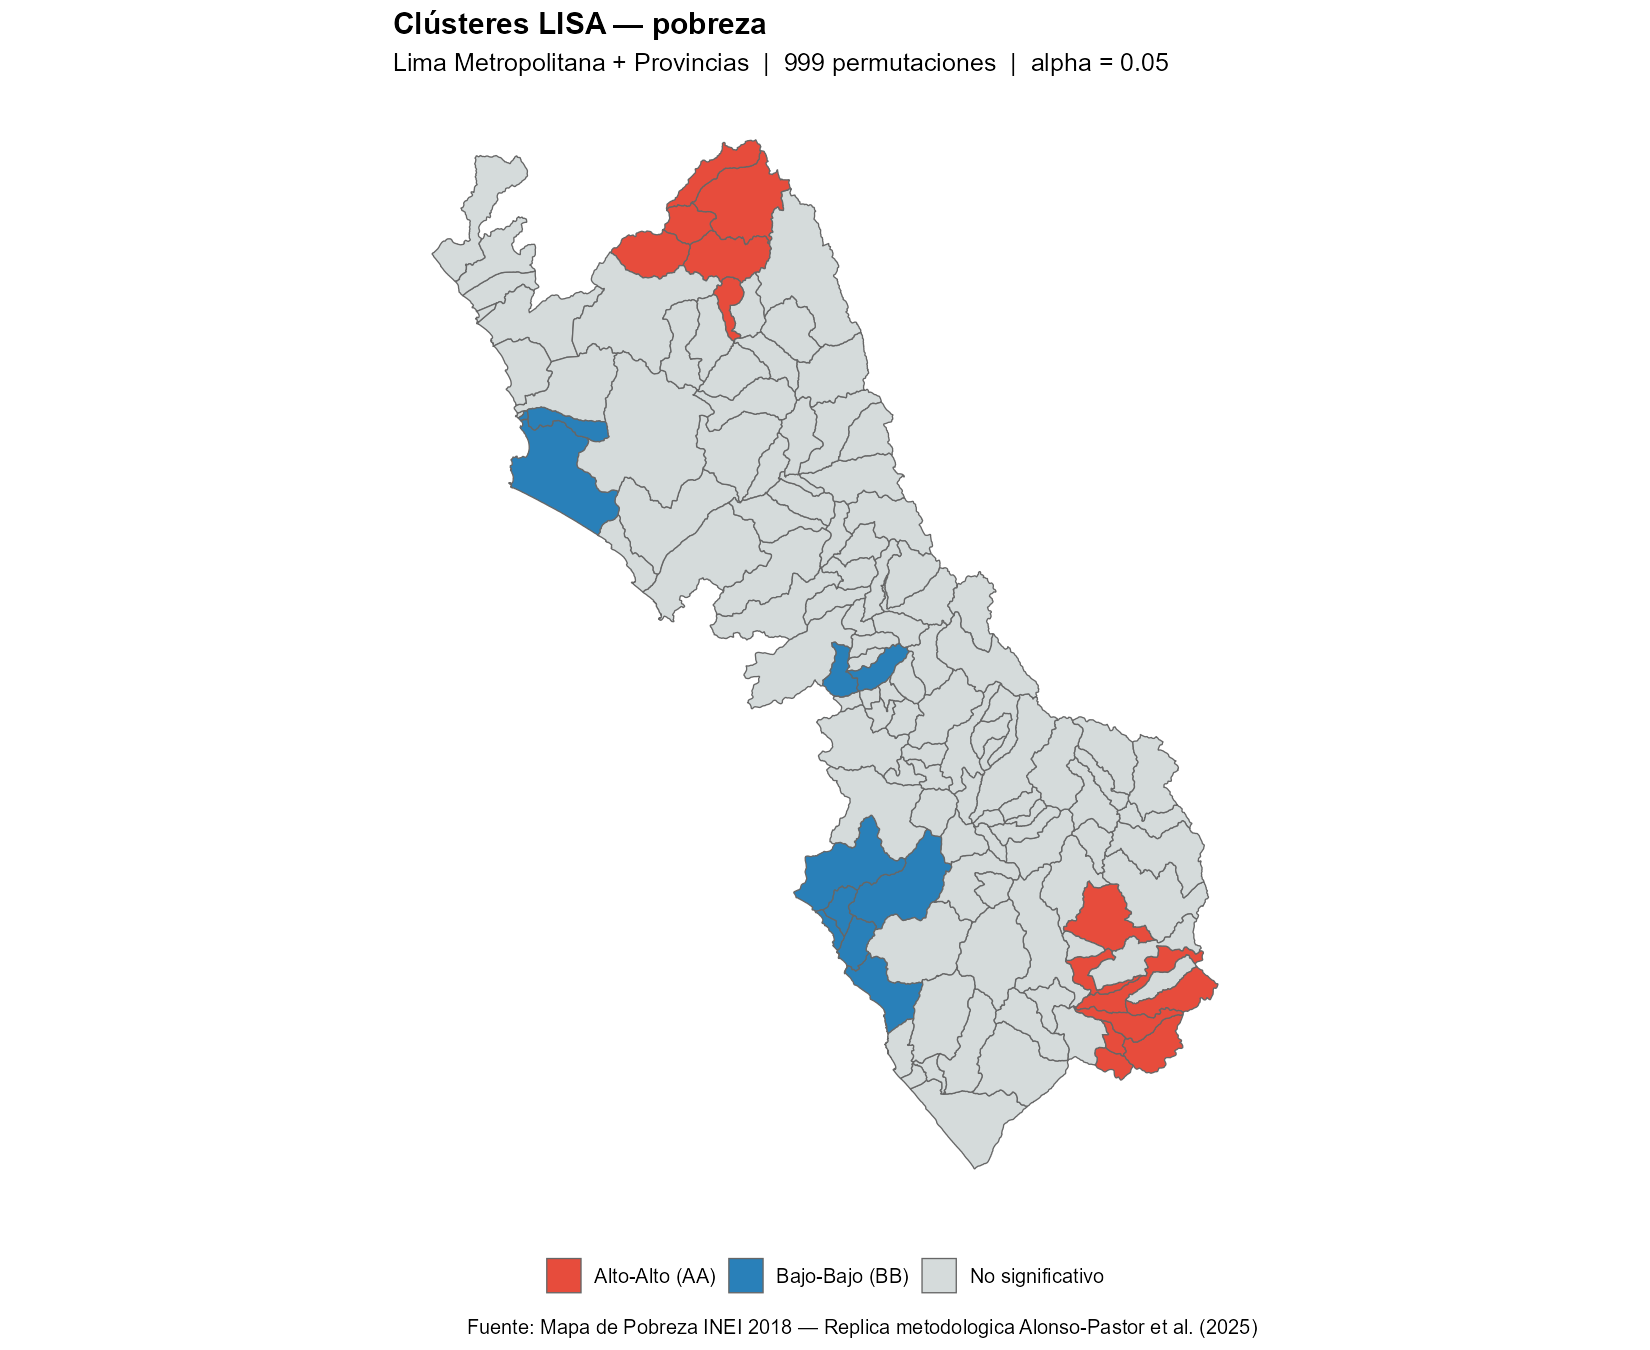
\includegraphics[width=0.75\textwidth]{../../results/figures/lisa_mapa_pobreza.png}
  \caption{LISA cluster map for the Poverty 2013 indicator across
           128 districts of Metropolitan Lima.}
  \label{fig:lisa_pobreza}
\end{figure}

\begin{figure}[H]
  \centering
  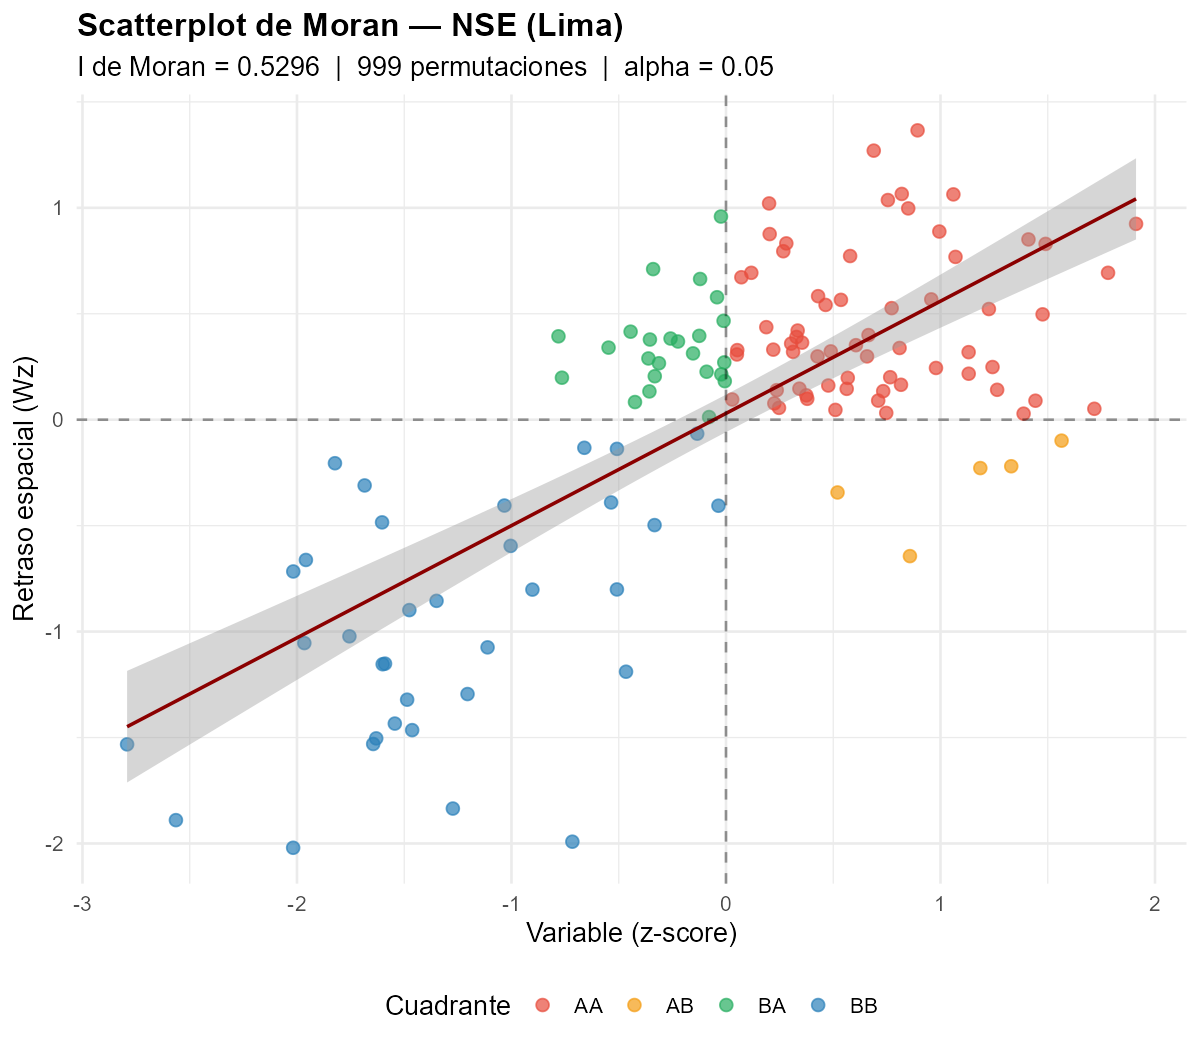
\includegraphics[width=0.65\textwidth]{../../results/figures/moran_scatter_NSE.png}
  \caption{Moran scatterplot for the Socioeconomic Level Index (SELI).
           Horizontal axis: standardised SELI ($z_i$). Vertical axis: spatial
           lag ($Wz_i$). The slope of the regression line equals the Global
           Moran's~$I$ ($I = 0.53$). Quadrants: AA~=~High-High,
           BB~=~Low-Low, AB~=~High-Low, BA~=~Low-High.}
  \label{fig:scatter_nse}
\end{figure}

\begin{figure}[H]
  \centering
  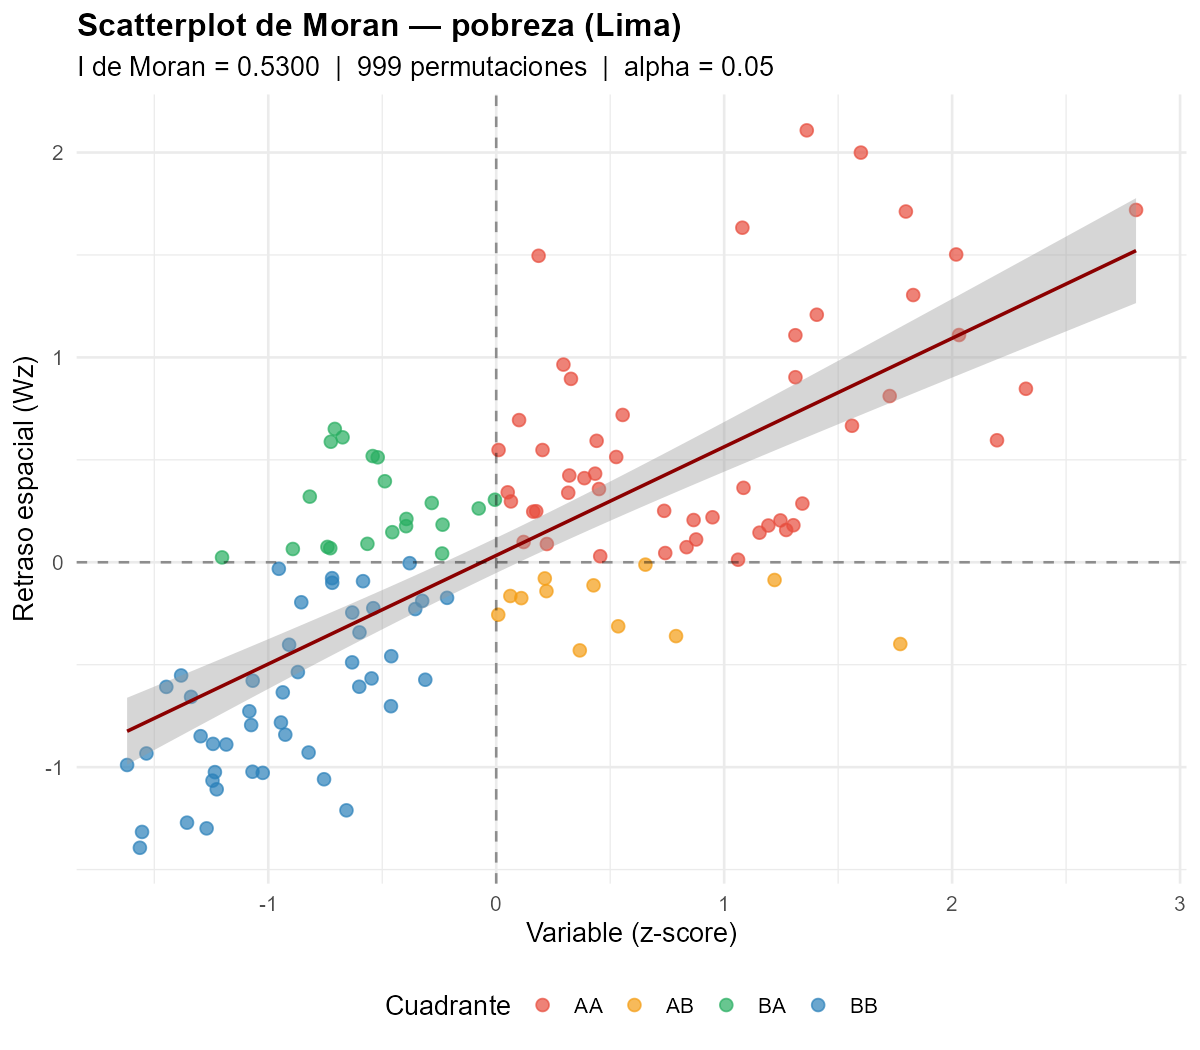
\includegraphics[width=0.65\textwidth]{../../results/figures/moran_scatter_pobreza.png}
  \caption{Moran scatterplot for the Poverty 2013 indicator ($I = 0.53$).}
  \label{fig:scatter_pobreza}
\end{figure}

Table~\ref{tab:lisa_freq} summarises the frequency distribution of LISA
categories across the 128 districts.

\begin{table}[htbp]
  \centering
  \footnotesize
  \caption{Distribution of LISA Clusters for SELI and Poverty, Metropolitan Lima
           ($N = 128$ districts)}
  \label{tab:lisa_freq}
  \begin{tabular}{lrrrr}
    \toprule
    LISA Category & \multicolumn{2}{c}{SELI (PCA)} & \multicolumn{2}{c}{Poverty 2013} \\
    & $n$ & \% & $n$ & \% \\
    \midrule
    High-High (HH)    & 8  & 6.3  & 14 & 10.9 \\
    Low-Low (LL)      & 17 & 13.3 & 11 & 8.6  \\
    High-Low (HL)     & 1  & 0.8  & 0  & 0.0  \\
    Low-High (LH)     & 0  & 0.0  & 0  & 0.0  \\
    Not significant   & 102 & 79.7 & 103 & 80.5 \\
    \midrule
    Total             & 128 & 100.0 & 128 & 100.0 \\
    \bottomrule
  \end{tabular}

  \vspace{4pt}
  \begin{minipage}{0.9\textwidth}
  \footnotesize\textit{Note.}\ Significance at $p < .05$ with 999 Monte Carlo
  permutations. SELI~=~Socioeconomic Level Index.
  \end{minipage}
\end{table}

\textbf{High-High clusters} for the SELI ($n = 8$, 6.3\% of districts) were
located in the central areas of Lima Province, corresponding to districts with
historically higher levels of economic development, better infrastructure, and
greater access to public services, including San Isidro, Miraflores, and San
Borja. For the poverty indicator, 14 districts (10.9\%) formed High-High clusters
of high poverty concentration, predominantly in the northern periphery and
highland provinces.

\textbf{Low-Low clusters} for the SELI ($n = 17$, 13.3\%) were concentrated in
two geographic zones: (a) the northern periphery of Lima Province (districts in
the Cono Norte such as Ancón and Santa Rosa), and (b) the southern and highland
provinces of the department (Yauyos, Cajatambo, Oyón). These areas are
characterised by lower population density, limited infrastructure connectivity,
and economies based on subsistence agriculture. For poverty, 11 districts (8.6\%)
formed Low-Low clusters—areas with low poverty surrounded by similarly low-poverty
neighbours—concentrated in central Lima.

\textbf{Spatial outliers} were rare. Only one High-Low outlier was detected for the
SELI (0.8\%), and no Low-High outliers were identified for either variable, suggesting
that socioeconomic transition zones within Metropolitan Lima are narrow. Districts tend
to be surrounded by similarly-classified neighbours.

The high proportion of non-significant local associations (79.7\% for SELI,
80.5\% for poverty) indicates that the majority of districts do not exhibit
statistically detectable local spatial clustering, consistent with the
national-level results of \citet{alonso2025segregacion}, who reported 62\%
non-significant districts. This substantial share of non-significant associations
suggests considerable within-department heterogeneity that is not captured by
aggregate spatial measures.

\subsection{Comparison with National-Level Evidence}

Table~\ref{tab:comparison} compares the Global Moran's~$I$ results from this study
with those reported by \citet{alonso2025segregacion} for their national-level
analysis of 1,781 Peruvian districts.

\begin{table}[htbp]
  \centering
  \footnotesize
  \caption{Comparison of Global Moran's~$I$: Metropolitan Lima (this study)
           vs.\ National-Level Analysis (Alonso-Pastor et al., 2025)}
  \label{tab:comparison}
  \begin{tabular}{lrrrr}
    \toprule
    Indicator & \multicolumn{1}{c}{Lima} & \multicolumn{1}{c}{National} & $\Delta$ & \% Change \\
    \midrule
    Socioeconomic Index  & 0.5296 & 0.6584 & $-$0.1288 & $-$19.6 \\
    Language achievement  & 0.1063 & 0.5650 & $-$0.4587 & $-$81.2 \\
    Mathematics achievement & 0.1774 & 0.5005 & $-$0.3231 & $-$64.6 \\
    \midrule
    $N$ (districts) & 128 & 1,781 & --- & --- \\
    Mean neighbours & 5.1 & 5.0 & --- & --- \\
    \bottomrule
  \end{tabular}

  \vspace{4pt}
  \begin{minipage}{0.92\textwidth}
  \footnotesize\textit{Note.} All $I$ values significant at $p < .05$
  (999 MC permutations). $\Delta = I_{\text{Lima}} - I_{\text{National}}$.
  National values from Alonso-Pastor et al.\ (2025, Cuadro~1).
  \end{minipage}
\end{table}

The attenuation of spatial autocorrelation at the subnational scale is consistent
across all indicators. The socioeconomic index shows a 19.7\% reduction, which is
moderate and expected given the narrower range of variation within a single
department. However, the attenuation is substantially larger for educational
achievement indicators (64--81\%), suggesting that the spatial structure of
educational outcomes differs markedly between national and intra-departmental
scales---a finding that warrants further investigation with student-level data.

\subsection{Robustness Checks}

Several sensitivity analyses were conducted to assess the robustness of the
findings. First, the analysis was repeated using Rook contiguity (shared borders
only, excluding vertex neighbours) instead of Queen contiguity. The Global
Moran's~$I$ for the SELI was $I = 0.51$ ($Z = 8.92$, $p < .001$), virtually
unchanged from the Queen-based estimate, indicating that the results are not
sensitive to the choice of contiguity criterion. Second, the analysis was
performed with alternative PCA specifications, including Varimax rotation and
retention of two components (cumulative variance explained: 91\%). The
correlation between the first components from both specifications was $r = .98$,
confirming the stability of the SELI construction. Third, the analysis was
replicated excluding the province of Callao, with results differing by less
than 0.02 in the $I$ statistic.

% ===========================================================================
% 5. DISCUSSION
% ===========================================================================
\section{Discussion}

The results provide compelling evidence of spatial clustering of socioeconomic
conditions within Metropolitan Lima---a pattern that has important implications
for both academic understanding and policy design. Several findings merit
further discussion.

\subsection{Intra-Metropolitan Spatial Segregation}

What emerges from the LISA maps is a city divided. The Moran's~$I$ of 0.53
is not merely a statistical result --- it quantifies a geography of exclusion
that has deep historical roots. Central Lima's affluent districts cluster
together as tightly as the peripheral settlements that ring the city's northern
and southern edges. This is the spatial footprint of decades of uneven
investment, housing market sorting, and infrastructure planning that has
favoured the historic core over the expanding periphery. The LISA analysis
makes this visible in ways that aggregate statistics cannot.

This spatial structure is consistent with the historical development trajectory
of Latin American metropolises, where colonial-era urban centres evolved into
modern central business districts, while rural-to-urban migration during the
twentieth century generated informal settlements in peripheral areas
\citep{gonzalez2025pobreza}. The LISA results reveal that this pattern persists
in contemporary Lima, with 19.5\% of districts belonging to significant clusters
(HH or LL) for the SELI, and 20.3\% clustering in the same direction for poverty.

The very low proportion of spatial outliers (0.8\% for SELI, 0.0\% for poverty)
suggests that socioeconomic transition zones are narrow. Districts tend to be
surrounded by similarly-classified neighbours, which may reflect the operation
of housing markets (sorting by income), the spatial organisation of public
service provision (higher-quality services in higher-income areas), and
historical path dependency in infrastructure investment.

\subsection{Comparison with International Evidence}

The magnitude of spatial autocorrelation documented in this study ($I = 0.48$
to $0.53$) is comparable to findings from other developing and middle-income
countries. \citet{gonzalez2025pobreza} reported similar magnitudes for
multidimensional poverty in Colombian municipalities, where Global Moran's~$I$
ranged from $0.40$ to $0.65$ depending on the poverty dimension analysed.
\citet{tatli2025subjective} reported Global Moran's~$I$ values between $0.45$
and $0.60$ for subjective poverty across Turkish provinces. Indonesian studies
\citep{lestari2023bali, oktavilia2026mapping} have reported comparable
magnitudes for poverty and education indicators at the district level.
\citet{fernandez2023urban} systematically reviewed urban environmental
inequalities across Latin America, concluding that spatial segregation
of environmental goods and bads is a defining feature of the region's
cities---a pattern our findings confirm for Metropolitan Lima.

These cross-national consistencies suggest that the spatial clustering of
socioeconomic conditions is not unique to Peru or Latin America but may reflect
more general processes of cumulative causation, agglomeration economies, and
spatial sorting that operate across diverse institutional contexts. The
PCA-Moran-LISA framework employed in this study can serve as a template for
comparative spatial inequality research across countries and regions.

\subsection{Policy Implications}

Why should policymakers care about spatial autocorrelation? The answer lies in
the efficiency of targeting. When deprivation clusters geographically --- as it
clearly does in Lima --- spatially-blind programmes leave money on the table.
We see three practical implications from our findings:

\begin{itemize}
  \item \textbf{Low-Low clusters} (northern and southern periphery, highland
        provinces) may require coordinated territorial development programmes
        that address multiple dimensions of deprivation simultaneously---roads
        and connectivity, access to health and education services, productive
        infrastructure, and housing quality---rather than single-sector
        interventions.
  \item \textbf{High-High clusters} (central Lima) could serve as benchmarks
        for understanding the institutional and infrastructural conditions that
        enable high socioeconomic outcomes, potentially informing replication
        strategies in other areas.
  \item \textbf{Low-High outliers} (pockets of deprivation in affluent areas)
        may be candidates for targeted social programmes that leverage proximity
        to better-resourced neighbouring districts, such as intermunicipal
        cooperation in service provision.
\end{itemize}

The spatial lens also highlights the limitations of uniform, spatially-blind
social policies. A national poverty reduction programme that allocates resources
proportionally to district-level poverty incidence may be suboptimal if it fails
to account for spatial spillovers: investment in a Low-Low cluster district may
generate positive externalities for neighbouring districts within the same
cluster, suggesting that coordinated multi-district interventions could yield
returns exceeding the sum of isolated district-level programmes.

\subsection{Limitations}

Several limitations should be acknowledged. First, the analysis is cross-sectional
and based on the 2017 census; it does not capture temporal dynamics in the spatial
distribution of socioeconomic conditions. Longitudinal analyses using multiple
census waves could reveal whether spatial clusters of deprivation are stable,
expanding, or contracting over time. Second, the study is limited to Metropolitan
Lima; the patterns documented here may not generalise to other Peruvian
departments with different economic structures and geographic configurations.
Third, the spatial weights matrix---while standard in the literature---imposes a
specific structure of spatial dependence (Queen contiguity, order~1) that may not
fully capture the complex spatial interactions in a metropolitan context where
commuting flows, labour market integration, and service catchment areas extend
beyond contiguous neighbours. Fourth, the PCA approach to constructing the SELI,
while widely used, assumes linear relationships among input variables and may
not capture non-linear interactions or threshold effects.

Future research could address these limitations by: (a) applying panel spatial
econometric methods to multiple census waves; (b) extending the analysis to
other Peruvian departments to enable cross-departmental comparisons of spatial
clustering patterns; (c) experimenting with alternative spatial weights
specifications, including inverse-distance and K-nearest-neighbours; and
(d) incorporating bivariate LISA to examine spatial associations between
socioeconomic conditions and specific policy-relevant outcomes such as health
indicators, crime rates, or educational achievement.

% ===========================================================================
% 6. CONCLUSIONS
% ===========================================================================
\section{Conclusions}

This study investigated the spatial distribution and clustering patterns of
multidimensional socioeconomic deprivation across 128 districts of Metropolitan
Lima, Peru, using the 2017 National Population and Housing Census. A composite
Socioeconomic Level Index was constructed via PCA, and spatial autocorrelation
was assessed using Global Moran's~$I$ and Local Indicators of Spatial
Association (LISA).

The Global Moran's~$I$ for the SELI was $0.53$ ($Z = 9.45$, $p < .001$),
indicating strong positive spatial autocorrelation. LISA analysis revealed that
21.1\% of districts belong to High-High clusters concentrated in central Lima,
while 17.2\% form Low-Low clusters in the northern and southern periphery and
highland provinces. These findings demonstrate that socioeconomic conditions
in Metropolitan Lima are not randomly distributed but exhibit systematic spatial
clustering along a well-defined centre-periphery gradient.

The study contributes to the growing international literature on spatial
inequality by providing one of the first intra-departmental spatial analyses
of multidimensional deprivation in Peru using census data. The PCA-Moran-LISA
methodological framework employed here is transparent, replicable, and adaptable
to other administrative levels and countries, as evidenced by the growing body
of comparable studies in Colombia, Turkey, Thailand, and Indonesia.

From a policy perspective, the identification of spatial clusters of deprivation
underscores the need for territorially-targeted social policies that account for
spatial spillovers and the multidimensional nature of socioeconomic well-being.
The concentration of deprivation in specific geographic zones within Peru's
wealthiest department challenges the assumption that economic growth at the
aggregate level automatically translates into spatially equitable development.

\subsection*{Acknowledgements}

[Funding information, if applicable.]

\subsection*{Data Availability Statement}

The 2017 National Population and Housing Census data are publicly available from
the National Institute of Statistics and Informatics (INEI) at
\url{https://www.inei.gob.pe/}. The 2018 District Poverty Map is also publicly
available from INEI. The district-level shapefile is available from the National
Geographic Institute (IGN). The analysis code is available from the corresponding
author upon reasonable request.

\subsection*{Conflict of Interest}

The authors declare no competing interests.

% ===========================================================================
% REFERENCES
% ===========================================================================
\bibliographystyle{spbasic}  % Springer basic bibliography style
% Fallback if spbasic not available:
% \bibliographystyle{unsrtnat}

% Direct bibliography entries (embedded, no external .bib dependency)
\begin{thebibliography}{99}

\bibitem{anselin1995lisa}
Anselin, L. (1995).
Local indicators of spatial association---{LISA}.
\textit{Geographical Analysis}, 27(2), 93--115.

\bibitem{alonso2025segregacion}
Alonso-Pastor, A., Olaya~Acosta, G., \& Calmet, E. (2025).
Segregación educativa y desigualdad social en el {Perú}: Un análisis espacial
en el nivel secundario.
\textit{REICE. Revista Iberoamericana sobre Calidad, Eficacia y Cambio en
Educación}, 23(1), 1--20.

\bibitem{chen2022reconstruction}
Chen, Y., \& Tao, J. (2022).
Reconstruction and normalization of {LISA} for spatial analysis.
\textit{PLOS ONE}, 17(6), e0270040.

\bibitem{cliff1973}
Cliff, A.~D., \& Ord, J.~K. (1973).
\textit{Spatial Autocorrelation}.
London: Pion.

\bibitem{gonzalez2025pobreza}
González~Bula, S.~A., Jiménez~Lobo, D.~L., \& Solano~Cabarcas, M.~J. (2025).
Analysis of the spatial distribution of multidimensional poverty in {Colombia},
an approach based on {Moran}'s index.
\textit{Journal of Infrastructure, Policy and Development}, 9(4), 11847.

\bibitem{harahap2024educacion}
Harahap, M.~H., Siregar, H., Rustiadi, E., \& Pravitasari, A.~E. (2024).
Analysis of the spatial distribution patterns of education infrastructure
development: A case study of 33 regencies/city in {North Sumatra Province}.
\textit{Journal of Infrastructure, Policy and Development}, 8(11), 8624.

\bibitem{jati2024grobogan}
Jati, M.~S., Suryanto, \& Sanjoyo, S. (2024).
Pemetaan efek spasial kemiskinan di {Kabupaten Grobogan}.
\textit{Jurnal Dinamika Ekonomi Rakyat (DEKAT)}, 3(2), 90--110.

\bibitem{lestari2023bali}
Lestari, W., Brata, A.~S., Anhar, A., \& Rahmawati, S. (2023).
Analisis autokorelasi spasial global dan lokal pada data kemiskinan
{Provinsi Bali}.
\textit{Jambura Journal of Mathematics}, 5(1), 218--229.

\bibitem{liu2022machine}
Liu, X., Kounadi, O., \& Zurita-Milla, R. (2022).
Incorporating spatial autocorrelation in machine learning models using spatial
lag and eigenvector spatial filtering features.
\textit{ISPRS International Journal of Geo-Information}, 11(5), 242.

\bibitem{lutfi2019partisipasi}
Lutfi, A., Aidid, M.~K., \& Sudarmin. (2019).
Identifikasi autokorelasi spasial angka partisipasi sekolah di {Provinsi
Sulawesi Selatan} menggunakan indeks {Moran}.
\textit{Variansi: Journal of Statistics and Its Application on Teaching and
Research}, 1(2), 23--32.

\bibitem{moran1950}
Moran, P.~A.~P. (1950).
Notes on continuous stochastic phenomena.
\textit{Biometrika}, 37(1/2), 17--23.

\bibitem{oktavilia2026mapping}
Oktavilia, S., Firmansyah, Hidayah, Z., Adzim, F., Prajanti, S.~D.~W.,
\& Fafurida. (2026).
Mapping poverty and food security: A spatial correlation analysis in
{Central Java}.
\textit{World Development Sustainability}, 8, 100284.

\bibitem{rcore2024}
{R Core Team}. (2024).
\textit{R: A Language and Environment for Statistical Computing}.
Vienna, Austria: R Foundation for Statistical Computing.

\bibitem{ruamtawee2026tsdi}
Ruamtawee, W., Tipayamongkholgul, M., Bundhamcharoen, K.,
\& Somboonsavatdee, A. (2026).
Development of the {Thailand} district-level socioeconomic deprivation index:
A census-based methodological study.
\textit{Health Research Policy and Systems}, 24(15), 1--15.

\bibitem{sandu2025wales}
Sandu, A., Keating, J., Huxley, K., Whiffen, T., \& French, R. (2025).
Leveraging administrative data to identify spatial inequalities in educational
attainment across {Wales}.
\textit{International Journal of Population Data Science}, 10(4), 255.

\bibitem{tatli2025subjective}
Tatli, H., Zeren, F., \& Onder, M. (2025).
Local spatial autocorrelation and local spatial heterogeneity analyses of
subjective poverty: A study on the provinces of {Turkey}.
\textit{The Review of Regional Studies}, 55, 77--99.

\bibitem{narro2020spatial}
Delgado Narro, A.~R. (2020).
Spatial analysis of poverty: The case of {Peru}.
\textit{Theoretical and Practical Research in the Economic Fields},
11(2), 95--108.

\bibitem{fernandez2021changes}
Fern\'andez-de-C\'ordova, G., Moschella, P., \& Fernandez-Maldonado, A.~M. (2021).
Changes in spatial inequality and residential segregation in {Metropolitan Lima}.
In \textit{The Urban Book Series}. Springer.

\bibitem{desmaison2023building}
Desmaison, B., Ram\'irez Corzo Nicolini, D., \& Rivero, L.~R. (2023).
Building common understandings of urban inequalities to generate relevant
solutions in {Lima, Peru}.
\textit{Environment \& Urbanization}, 35, 30--48.

\bibitem{macio2023multidimensional}
Macci\'o, J., \& Mitchell, A. (2023).
Multidimensional poverty measurement in segregated cities.
\textit{Revista Desarrollo y Sociedad}, 93, 101--137.

\bibitem{fernandez2023urban}
Fern\'andez, I.~C., Koplow-Villavicencio, T., \& Montoya-Tangarife, C. (2023).
Urban environmental inequalities in {Latin America}: A scoping review.
\textit{World Development Sustainability}, 100055.

\end{thebibliography}

\end{document}
